%%%%%%%%%%%%%%%%%%%%%%%%%%%%%%%%%%%%%%%%%%%%%%%%%%%%%%%%%%%%%%%%%%%%%%%%%%%%%%%%%%%
%% This project aims to create the UFC template for presentation.                %%
%% author: Maurício Moreira Neto - Doctoral student in Computer Science (MDCC)   %%
%% contacts:                                                                     %%
%%    e-mail: maumneto@ufc.br                                                    %%
%%    linktree: https://linktr.ee/maumneto                                       %%
%%%%%%%%%%%%%%%%%%%%%%%%%%%%%%%%%%%%%%%%%%%%%%%%%%%%%%%%%%%%%%%%%%%%%%%%%%%%%%%%%%%
\documentclass{libs/ufc_format}
% Inserting the preamble file with the packages
%%%%%%%%%%%%%%%%%%%%%%%%%%%%%%%%%%%%%%%%%%%%%%%%%%%%%%%%%%%%%%%%%%%%%
%% This file contains the packages that can be used in the beamer. %%
%%%%%%%%%%%%%%%%%%%%%%%%%%%%%%%%%%%%%%%%%%%%%%%%%%%%%%%%%%%%%%%%%%%%%
% Package to fonts family
\usepackage[T1]{fontenc}
% Package to accentuation
\usepackage[utf8]{inputenc}
% Package to Portuguese language
\usepackage[brazil]{babel}
% Package to Figures
\usepackage{graphicx}
% Package to the colors
\usepackage{color}
% Package to the colors
\usepackage{xcolor}
% Packages to math symbols and expressions
\usepackage{amsfonts, amssymb, amsmath}
% Package to multiple lines and columns in table
\usepackage{multirow, array} 
% Package to create pseudo-code
% For more detail of this package: http://linorg.usp.br/CTAN/macros/latex/contrib/algorithm2e/doc/algorithm2e.pdf
\usepackage{algorithm2e}
% Package to insert code
\usepackage{listings} 
\usepackage{keyval}
% Package to justify text
\usepackage[document]{ragged2e}
% Package to manage the bibliography
\usepackage[backend=biber, style=numeric, sorting=none]{biblatex}
% Package to facilities quotations
\usepackage{csquotes}
% Package to use multicols
\usepackage{multicol}

% Packages added by me
\usepackage{url}
\usepackage{tikz}
%\usepackage{multimedia}
%\usepackage{media9}[playbutton=plain, windowed=1280x720]
% Inserting the references file
\bibliography{references.bib}
\renewcommand*{\bibfont}{\scriptsize}

% Title
\title[ML]{\huge\textbf{Redes de Computadores}}
% Subtitle
\subtitle{Parte 3}
% Author of the presentation
\author{Evandro J.R. Silva}
% Institute's Name
\institute[Estácio Teresina]{
    % email for contact
    \normalsize{\email{ejrs.profissional@gmail.com}}
    \newline
    % Department Name
    \department{Bacharelado em Ciência da Computação}
    \newline
    % university name
    %\ufc
    \estaciothe
}
% date of the presentation
\date{05 a 06 de Agosto}


%%%%%%%%%%%%%%%%%%%%%%%%%%%%%%%%%%%%%%%%%%%%%%%%%%%%%%%%%%%%%%%%%%%%%%%%%%%%%%%%%%
%% Start Document of the Presentation                                           %%               
%%%%%%%%%%%%%%%%%%%%%%%%%%%%%%%%%%%%%%%%%%%%%%%%%%%%%%%%%%%%%%%%%%%%%%%%%%%%%%%%%%
\begin{document}
% insert the code style
%%%%%%%%%%%%%%%%%%%%%%%%%%%%%%%%%%%%%%%%%%%%%%%%%%%%%%%%%%%%%%%%%%%%%%%%%%%%%%%%%%%
%% This file contains the style of the codes show in slides.                     %%
%% The package used is listings, but it possible to used others.                 %%
%%%%%%%%%%%%%%%%%%%%%%%%%%%%%%%%%%%%%%%%%%%%%%%%%%%%%%%%%%%%%%%%%%%%%%%%%%%%%%%%%%%

% color used in the code style
\definecolor{codegreen}{rgb}{0,0.6,0}
\definecolor{codegray}{rgb}{0.5,0.5,0.5}
\definecolor{codepurple}{rgb}{0.58,0,0.82}
\definecolor{codebackground}{rgb}{0.95,0.95,0.92}

% style of the code!
\lstdefinestyle{codestyle}{
    backgroundcolor=\color{codebackground},   
    commentstyle=\color{codegreen},
    keywordstyle=\color{magenta},
    numberstyle=\tiny\color{codegray},
    stringstyle=\color{codepurple},
    basicstyle=\ttfamily\footnotesize,
    frame=single,
    breakatwhitespace=false,         
    breaklines=true,                 
    captionpos=b,                    
    keepspaces=true,                 
    numbers=left,                    
    numbersep=5pt,                  
    showspaces=false,                
    showstringspaces=false,
    showtabs=false,                  
    tabsize=2,
    title=\lstname 
}

\lstset{style=codestyle}


%% ---------------------------------------------------------------------------
% First frame (with tile, subtitle, ...)
\begin{frame}{}
    \maketitle
\end{frame}

%% ---------------------------------------------------------------------------
% Second frame
\begin{frame}{Sumário}
    \begin{multicols}{2}
        \tableofcontents
    \end{multicols}
\end{frame}

%=============================================================================
% SECTION 5
%=============================================================================
\section{Camada de Rede}

%-----------------------------------------------------------------------------
% SUBSECTION 5.1
%-----------------------------------------------------------------------------
\subsection{IP}

\begin{frame}{}
    \centering
    \Large
    Camada de Rede\\
    \large
    Internet Protocol (IP) - Continuação
\end{frame}

\begin{frame}{Datagrama IPv4}
    \centering
    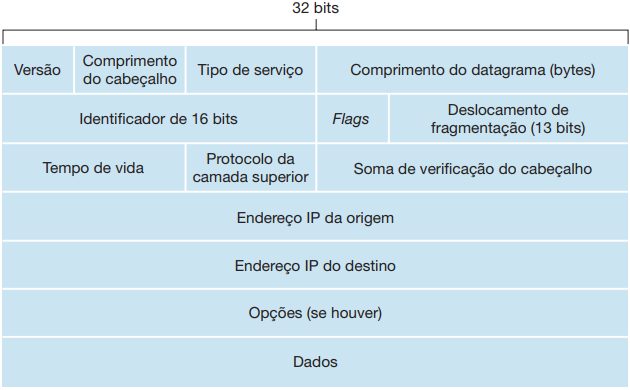
\includegraphics[scale=0.45]{figuras/figura10_01}
    \begin{itemize}
        \footnotesize
        \justifying
        \item \textbf{Número da versão}: quatro bits que identificam a versão do protocolo IP do datagrama. Ao analisar a versão o roteador saberá como interpretar o restante do datagrama.
        \item<2> \textbf{Comprimento do cabeçalho}: quatro bits que determinam \textit{onde} começam os dados no datagrama (uma vez que o cabeçalho tem comprimento variável). Porém, a maioria dos datagramas não utiliza as opções do cabeçalho e, portanto, um datagrama típico terá 20 bytes.
    \end{itemize}
\end{frame}

\begin{frame}{Datagrama IPv4}
    \begin{itemize}
        \justifying
        \item \textbf{Tipo de serviço}: bits que servem para diferenciar os tipos de datagrama. Por exemplo, um serviço de baixo atraso, alta vazão ou confiabilidade podem ser sinalizados aqui.
        \item<2-> \textbf{Comprimento do datagrama}: comprimento total do datagrama medido em bytes. Como são 16 bits, o tamanho \textbf{teórico} de um datagrama pode chegar a 65.535 bytes, mas na realidade poucos passam a marca de 1500 bytes.
        \item<3-> \textbf{Identificador}, \textbf{flags} e \textbf{deslocamento de fragmentação}: três campos relacionados à fragmentação do IP (possível no IPv4, mas não no IPv6).
        \item<4-> \textbf{Tempo de vida}: ou TTL (\textit{Time-To-Live}) é incluído para garantir que datagramas não fiquem circulando para sempre na rede. Cada vez que o datagrama passa por um roteador, o tempo de vida é decrementado. Quando o valor atinge 0, o datagrama é descartado.
    \end{itemize}
\end{frame}

\begin{frame}{Datagrama IPv4}
    \begin{itemize}
        \justifying
        \item \textbf{Protocolo}: quando o datagrama chega em seu destino final o valor desse campo indica o protocolo da camada de transporte ao qual os dados devem ser passados. A IANA definiu os números dos protocolos então, por exemplo, o número 6 indica o TCP, enquanto o número 17 indica o UDP.
        \item<2-> \textbf{Soma de verificação do cabeçalho}: auxilia um roteador na detecção de erros de bits em um datagrama recebido. Cada 2 bytes é tratado como se fosse um número, os quais são somados  usando complementos aritméticos de 1 (ou seja, o cálculo feito como o do \textit{checksum} do UDP).
        \item<3-> \textbf{Endereços IP de origem e destino}: quando o datagrama é criado, o endereço de origem e o de destino é inserido. O endereço de destino pode ser consultado, por exemplo, via DNS.
    \end{itemize}
\end{frame}

\begin{frame}{Fragmentação do Datagrama}
    \begin{itemize}
        \justifying
        \item Um datagrama é enviado para a camada de enlace onde vai ser encapsulado em um quadro.
        \item Os quadros possuem uma quantidade máxima de dados que podem transmitir (MTU - \textit{Maximum Transmission Unit}).
        \item Quando dividido, cada parte do datagrama é chamado de \textbf{fragmento}.
        \item<2-> Os fragmentos são marcados com o identificador do datagrama original.
        \item<3-> O último fragmento tem um bit de flag ajustado para 0, enquanto os demais possuem o flag ajustado para 1.
        \item<4-> O campo de deslocamento especifica a localização do fragmento no datagrama original.
    \end{itemize}
\end{frame}

\begin{frame}{Fragmentação do Datagrama}
\centering
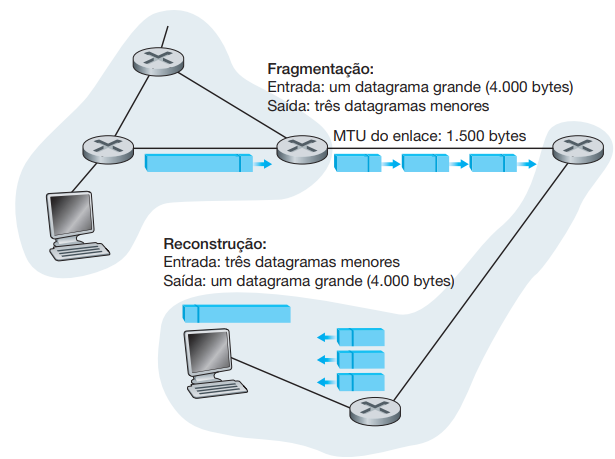
\includegraphics[scale=0.35]{figuras/figura10_02}\\
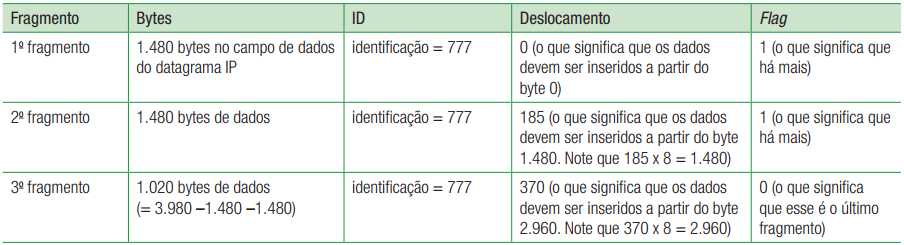
\includegraphics[scale=0.45]{figuras/figura10_03}
\end{frame}

%=============================================================================
% SECTION 6
%=============================================================================
\section{FIM}

\begin{frame}{}
    \centering
    \Large
    FIM!\\
    Obrigado pela atenção e paciência!
\end{frame}

%=============================================================================
% SECTION REFERENCES
%=============================================================================
%\begin{frame}[allowframebreaks]{Referências}
%    \scriptsize
%    \printbibliography
%\end{frame}

\end{document}













%% ---------------------------------------------------------------------------
% This presentation is separated by sections and subsections
%\section{Seção I}
%\begin{frame}{Explicações}
%    % itemize
%    Este é um template que pode ser utilizado para:
%    \begin{itemize}
%        \item Apresentação de Trabalhos Acadêmicos
%        \item Apresentação de Disciplinas
%        \item Apresentações de Teses e Dissertações
%    \end{itemize}
%
%    \vspace{0.4cm} % vertical space
%    
%    % enumeration
%    Para utilizar este template corretamente é importante que:
%    \begin{enumerate}
%        \item Tenha conhecimento mínimo sobre LaTeX
%        \item Ler os comentários no template (explicações)
%        \item Ler o README.md (documentação)
%    \end{enumerate}
%
%    \vspace{0.2cm}

%    \example{Este é um texto de exemplo!} \emph{Texto de Ênfase!}
%\end{frame}

%% ---------------------------------------------------------------------------
%\subsection{Subseção I}
%\begin{frame}{Criando Blocos}
%    % Blocks styles
%    \begin{block}{Bloco Padrão}
%        Texto do corpo do bloco.
%    \end{block}

%    \begin{alertblock}{Bloco de Alerta}
%        Texto do corpo do bloco.
%    \end{alertblock}
%
%    \begin{exampleblock}{Bloco de Exemplo}
%        Texto do corpo do bloco.
%    \end{exampleblock}   
%\end{frame}

%% ---------------------------------------------------------------------------
%\subsection{Subseção II}
%\begin{frame}{Criando Caixas}
%    \successbox{testando o success box}
%
%    \pause
%
%    \alertbox{testando o alert box}
%
%    \pause
%
%    \simplebox{testando o simple box}
%\end{frame}

%% ---------------------------------------------------------------------------
%\subsection{Subseção III}
%\begin{frame}{Criando Algoritmos (Pseudocódigo)}
%    \begin{algorithm}[H]
%        \SetAlgoLined
%        \LinesNumbered
%        \SetKwInOut{Input}{input}
%        \SetKwInOut{Output}{output}
%        \Input{x: float, y: float}
%        \Output{r: float}
%        \While{True}{
%          r = x + y\;
%          \eIf{r >= 30}{
%           ``O valor de $r$ é maior ou iqual a 10.''\;
%           break\;
%           }{
%           ``O valor de $r$ = '', r\;
%          }
%         } 
%         \caption{Algorithm Example}
%    \end{algorithm}
%\end{frame}

%% ---------------------------------------------------------------------------

%\begin{frame}{Inserindo Algoritmos}
%    \lstset{language=Python}
%    \lstinputlisting[language=Python]{code/main.py}
%\end{frame}

%% ---------------------------------------------------------------------------
%\begin{frame}{Inserindo Algoritmos}
%    \lstinputlisting[language=C]{code/source.c}
%\end{frame}

%% ---------------------------------------------------------------------------
%\begin{frame}{Inserindo Algoritmos}
%    \lstinputlisting[language=Java]{code/helloworld.java}
%\end{frame}

%% ---------------------------------------------------------------------------
%\begin{frame}{Inserindo Algoritmos}
%    \lstinputlisting[language=HTML]{code/index.html}
%\end{frame}

%% ---------------------------------------------------------------------------
% This frame show an example to insert multicolumns
%\section{Multicolunas}
%\begin{frame}{Seção II - Multicolunas}
%    \begin{columns}{}
%        \begin{column}{0.5\textwidth}
%            \justify
%            É possível colocar mais de uma coluna utilizando os comandos de $\backslash$begin\{column\}\{\} e $\backslash$end\{column\}
%        \end{column}
%        \begin{column}{0.5\textwidth}
%            \justify
%            Porém, o espaçamento deve ser proporcional entre as colunas para que estas colunas não entrem em coflito. O espaçamento é dado pelo segundo argumento do $\backslash$begin.
%        \end{column}
%    \end{columns}    
%\end{frame}

%% ---------------------------------------------------------------------------
% This frame show an example to insert figures
%\section{Imagens}
%\begin{frame}{Seção III - Figures}
%    \begin{figure}
%        \centering
%        \caption{Emblema da UFC.}
%        
\includegraphics[scale=0.3]{libs/emblemufc.pdf}
%        \source{Obtido pelo site oficial da UFC \cite{siteufc} \cite{einstein}}
%        \label{fig:ufc_emblem}
%    \end{figure}
%\end{frame}

%% ---------------------------------------------------------------------------
% Reference frames
%\begin{frame}[allowframebreaks]
%    \frametitle{Referências}
%    \printbibliography
%\end{frame}

%% ---------------------------------------------------------------------------
% Final frame
%\begin{frame}{}
%    \centering
%    \huge{\textbf{\example{Obrigado(a) pela Atenção!}}}
%    
%    \vspace{1cm}
%    
%    \Large{\textbf{Contato:}}
%    \newline
%    \vspace*{0.5cm}
%    \large{\email{usuario@dominio}}
%\end{frame}